\section{Resultados} \label{sec:result}
Neste capítulo é mostrado um breve resultado do que foi realizado até o presente momento.

\subsection{Planejamento do Problema} \label{subsec:planexp}

Assim como foi mostrado na seção \ref{subsubsec:etp} as etapas da dissertação, com isso cada modelo e os métodos que pode ser utilizado para responder as Questões de pesquisas abordado na seção \ref{subsubsec:obespec}. Com as etapas podemos dar uma cronologia logica do que foi adquirido ao longo do tempo com os dados da SANEPAR.

\subsubsection{Análise Exploratória dos dados (EDA)}

Da \ref{etp:1} é realizado o EDA para os processamento de dados que obteve até aqui, com o EDA vai ser respondido. Segundo \citeonline{Yu2016} Na era do big data, coletamos volumes de dados de massa caóticos, não estruturados e multimídia por meio de vários canais. Como descobrir as regras, os modelos analíticos e as hipóteses nesses dados tornou-se o novo desafio. A análise exploratória de dados foi promovida por John Tukey para incentivar os estatísticos a explorar os dados e, possivelmente, formular hipóteses que poderiam levar a uma nova coleta de dados e experimentos. Diferente da análise inicial de dados, a análise exploratória de dados (EDA) é uma abordagem para analisar conjuntos de dados para resumir suas principais características, muitas vezes com métodos visuais. Muitas técnicas de EDA foram adotadas na análise de big data.


Olhando para \ref{q1} relacionando a demanda com a variável que esta sendo prevista, e a pressão com a variável PT01 da Figura \ref{fig:person} pode se notar que ambas estão trabalhando por igual, quase uma correlação perfeita de $r=1$ então para essa questão basta olhar a correlação de Pearson na Figura \ref{fig:person}. 

Para \ref{q2} vai ser feito uma tabela para que seja respondido melhor essa questão

\begin{table}[H]
	\centering
	\caption{Descrição Estatística dos dados com filtro aplicado de 18 a 21h}\label{tb:est}
	\begin{tabular}{@{}cccccccccc@{}}
		\toprule
		\textbf{18 a 21h}  & \textbf{B1} & \textbf{B2} & \textbf{B3} & \textbf{LT01} & \textbf{FT01} & \textbf{FT02} & \textbf{FT03} & \textbf{PT01} & \textbf{PT02} \\ \midrule
		\textbf{Contagem} & 1096        & 1096        & 1096        & 1096          & 1096          & 1096          & 1096          & 1096          & 1096          \\
		\textbf{Média}    & 48,830      & 17,538      & 4,299       & 3,545         & 211,771       & 113,805       & 100,139       & 4,485         & 19,424        \\
		\textbf{STD}      & 12,354      & 9,282       & 8,976       & 0,438         & 44,496        & 21,486        & 19,822        & 0,487         & 4,323         \\
		\textbf{Min}      & 0,000       & 0,000       & 0,000       & 1,459         & 22,854        & 3,584         & 10,383        & 1,925         & 0,831         \\
		\textbf{25\%}     & 50,491      & 13,289      & 0,000       & 3,345         & 195,944       & 105,096       & 99,239        & 4,245         & 19,805        \\
		\textbf{50\%}     & 54,204      & 19,965      & 0,000       & 3,644         & 215,791       & 115,733       & 104,846       & 4,571         & 21,015        \\
		\textbf{75\%}     & 54,818      & 22,792      & 2,376       & 3,843         & 238,325       & 126,246       & 110,006       & 4,813         & 21,140        \\
		\textbf{Max}      & 57,885      & 53,488      & 46,841      & 4,256         & 301,863       & 181,565       & 143,988       & 5,475         & 23,679        \\ \bottomrule
	\end{tabular}

	Fonte: Elaboração própria a partir de dados da SANEPAR (2018 a 2020)
\end{table}

Na Tabela \ref{tb:est} o desvio padrão é dado pela sigla de STD que vem do inglês \textit{standard deviation}, observando também para responder a \ref{q2}, assim como toda companhia de tratamento de água é feito um acionamento automático, chamando de trava de segurança, para que o tanque não chegue a zerar e faltar água em todos os lugares adjacente que é abastecido por essa água, esse mínimo que o tanque pode chegar é de $1,459 m^3\Longleftrightarrow 1459 $ litros e as bombas serão acionadas em sua potencia máxima, para evitar o acionamento das bombas o nível do reservatório tem que estar no intervalo de $[3.843,4.256]\ m^3$ ainda sim, a bomba 1 estaria em funcionamento para completar o nível. Em casos de horários de picos o mais ideal, mas não o mais lucrativo é outro tanque de reserva nesses horários, e instalar uma tubulação para ligar um ao outro. Durante o dia estaria abastecendo os dois e a noite pela gravidade eles ficariam com o mesmo nível até o consumo chegar em um nível de acionamento das bombas.  

\begin{figure}[H]
	\centering
	\caption{Solução para acionamento das bombas}
	\label{fig:esquema}
	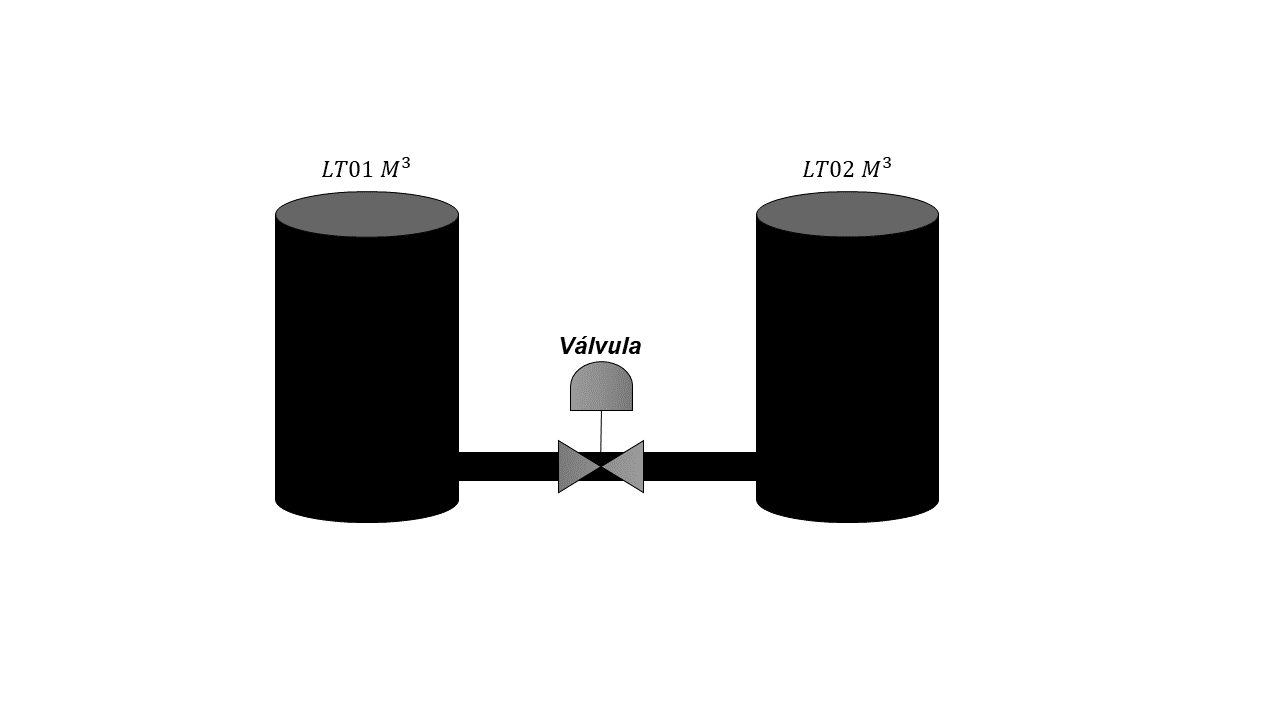
\includegraphics[width=1\linewidth]{Resultados/Figuras/esquema}
	Fonte: Elaboração própria 
\end{figure}

Na Figura \ref{fig:esquema} um esquema pratico para evitar a falta de água e o consumo em horários de pico. Esse esquema é bem simples de como pode ser melhorado o aproveitado de tempo no período do dia para armazenamento de água.

Na \ref{q3} o tanque tem como máximo nos dados $4,256 m^3$ dano em litros $4256$L para atender essa demanda e manter o tanque quase cheio ou sempre cheio, a Vasão de entrada tem que estar em $[238,302] \ m^3/h$, vasão de gravidade tem que ficar entre $[126,182] m^3/h$, vasão de recalque entre $[110,144] m^3/h$, pressão de sucção entre $[1.92,4.24] mca$ pressão de recalque entre $[21,24] mca$.

Na \ref{q4} o ponto de equilibro para não ser acionado as bomba seria de as vazão FT01 $211 m^3/h$  FT02 $114 m^3/h$ FT03 $100m^3/h$ e o nível do tanque com $3,545 m^3$.

Na \ref{q5:a} o tanque deve estar com o nível de $4,00 m^3$ para que não precise acionar bombas no horário de pico. 

\subsubsection{Múltiplas entradas e saída única (MISO)}

Nessa \ref{etp:2} o modelos que mais foi abordado no decorrer da dissertação é os modelos ARIMA, ou os que derivam desse modelo, e os modelos regressivo fora o LR  tem múltiplas entra e uma saída da variável que é prevista o LT01, as outras variáveis serve de apoio para melhorar os modelos do tipo ARX ou modelos com variáveis exógenas. Os modelos ARIMA sem a variável exógena é apenas um entrada, semelhante com o LR.



\subsubsection{Decomposição STL}

 \citeonline{Theodosiou20111178} A decomposição sazonal e tendencial utilizando o procedimento de Loess (STL) é utilizada para a decomposição aditiva da série temporal global. O STL realiza a decomposição aditiva dos dados por meio de uma sequência de aplicações do Loess mais suave, que aplica regressões polinomiais ponderadas localmente em cada ponto do conjunto de dados, sendo as variáveis explicativas os valores mais próximos do ponto cuja resposta está sendo estimada. 
 
 \begin{figure}[H]
 	\centering
 	\caption{Decomposição STL aditiva dos dados coletados}
 	\label{fig:stl-aditiva}
 	\includegraphics[width=1\linewidth]{"Resultados/Figuras/STL aditiva"}
 	
 	Fonte: Elaboração própria a partir de dados da SANEPAR (2018 a 2020)
 \end{figure}
 
 
 \begin{figure}[H]
 	\centering
 	\caption{Decomposição STL multiplicativa dos dados coletados}
 	\label{fig:stl}
 	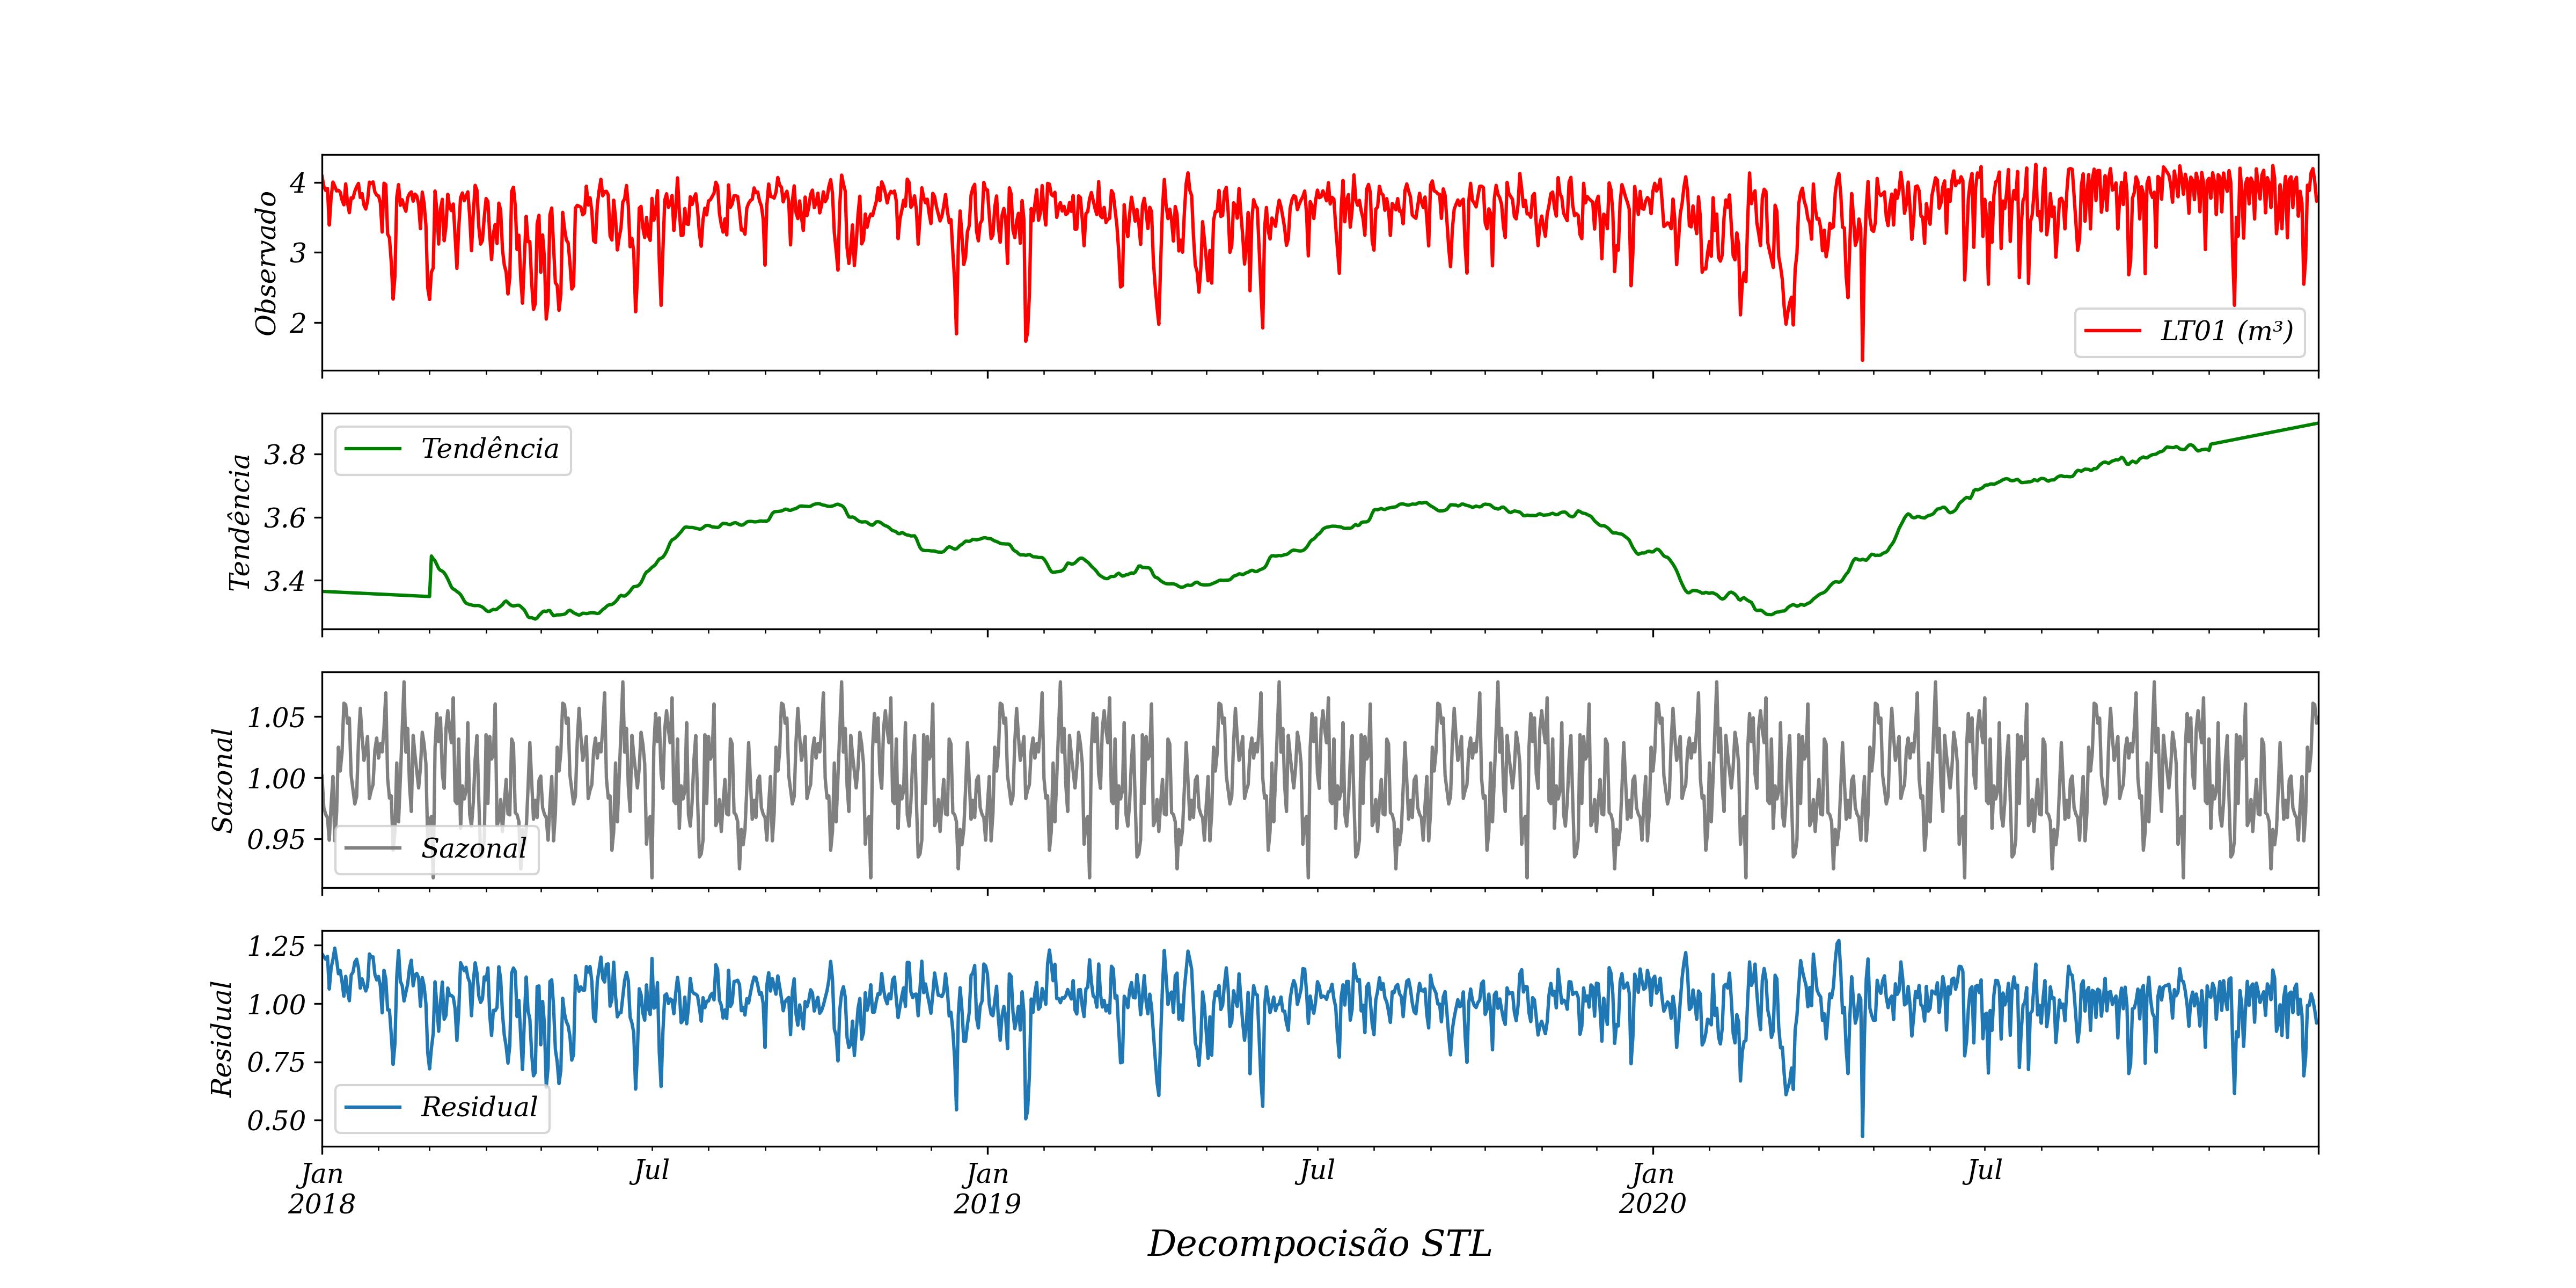
\includegraphics[width=1\linewidth]{Resultados/Figuras/STL}
 	
 	Fonte: Elaboração própria a partir de dados da SANEPAR (2018 a 2020)
 \end{figure}
 
 Na  \ref{q5}\ref{q5:b} pode ser respondida pela Figuras \ref{fig:stl-aditiva} e \ref{stl} como é observado tem tenência, sazonalidade e resido.
 
Na decomposição o objetivo dela é analisar se há tenência, sazonalidade e resido, olhando nas Figuras \ref{fig:stl} e \ref{fig:stl-aditiva}, isso mostra que os dados tem ambas das analise. E com isso perceber que a série é estacionaria, pelo teste a seguir.

Teste de Dickey-Fuller (DF) Aumentado: 
\begin{itemize}
	\item Estatística de teste ADF     $-4.248$
\item $p-valor$                       $0.001$
\item atrasos utilizados         $21.000$
\item  observações              $1074.000$
\item valor crítico $(1\%)           -3.436$
\item valor crítico $(5\%)           -2.864$
\item valor crítico $(10\%)          -2.568$


Fortes provas contra a hipótese nula

Rejeitar a hipótese nula

Os dados não têm raiz unitária e são estacionários, Na \ref{q5}\ref{q5:c} como a serie é estacionaria, para identificar quais os horários de pico entre as 18 até as 21h não é um trabalho fácil, pois se pegar na Figura \ref{fig:hist} pode perceber que no ano de 2020 teve um aumento da demanda nessas horas.

\begin{figure}[H]
	\centering
	\caption{Histograma do nível do reservatório}
	\label{fig:hist}
	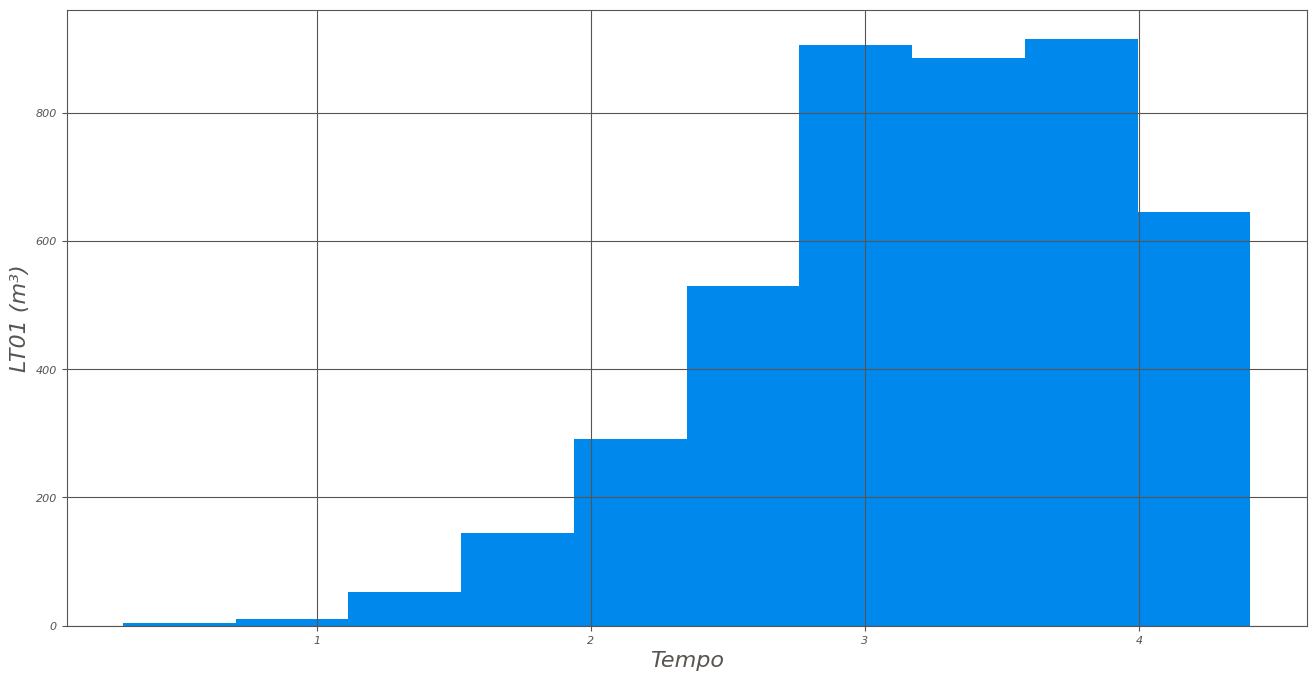
\includegraphics[width=1\linewidth]{Resultados/Figuras/hist}
	
	Fonte: Elaboração própria a partir de dados da SANEPAR (2018 a 2020)
\end{figure}

Então como dito na seção \ref{subsubsec:motivacao} as anomalias de tempo mais ocasionada no ano de 2020 e foi devido a falta de chuva nesse período.

Na \ref{q5}\ref{q5:d} nos horários de picos deve conter no tanque por volta de $[3.545,4.256] m^3$ para que não acione as bombas.

Para \ref{q5}\ref{q5:e} é mostrado na Figura \ref{fig:ft03} como pode ser afetado a vazão com o nível do tanque. A vazão de recalque influência mais no nível do tanque que as outras vazão pois injeta água no tanque por meio da bomba de recalque, que fica mais próximo da base do tanque, e as outras vazão por ter alguns valores ausente, não interfere tanto na amostra.

\begin{figure}[H]
	\centering
	\caption{Histograma da vazão de recalque}
	\label{fig:ft03}
	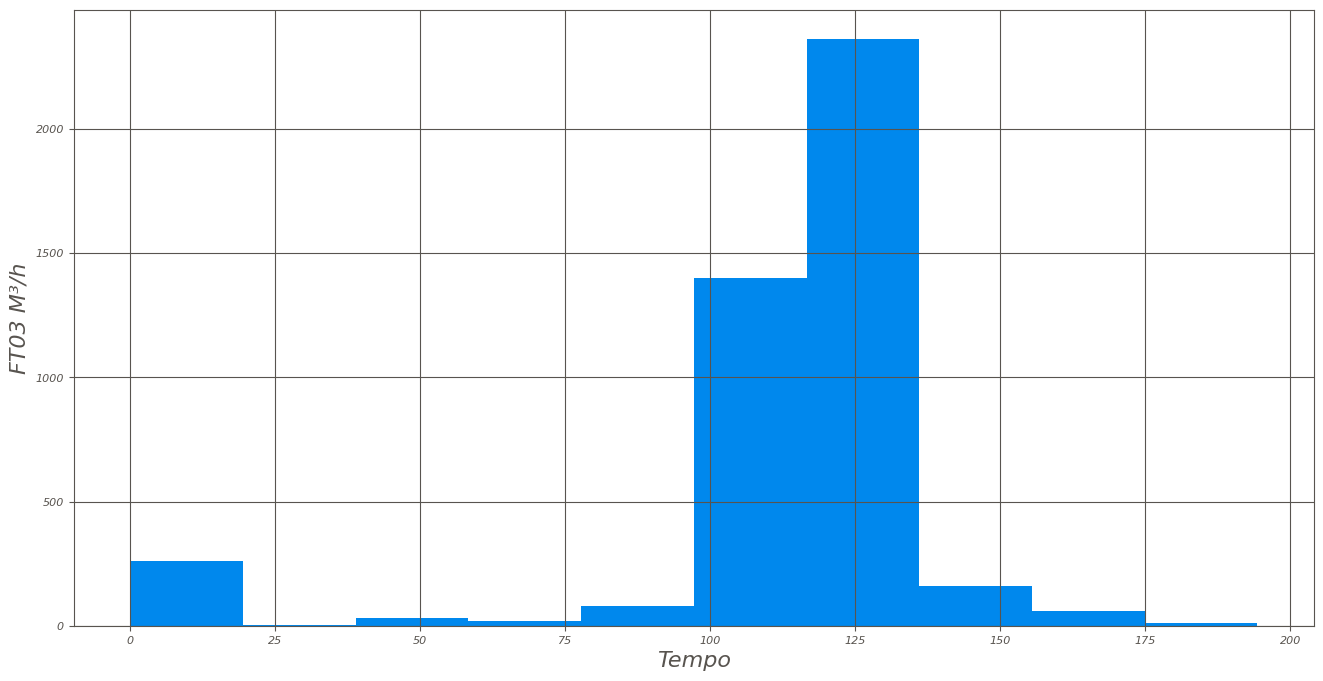
\includegraphics[width=1\linewidth]{Resultados/Figuras/ft03}
	
	Fonte: Elaboração própria a partir de dados da SANEPAR (2018 a 2020)
\end{figure}


\end{itemize}

Segundo  \citeonline{Reisen2017115} o teste de DF tem como formula a seguinte equações

\begin{eqnarray}
	z_t&=& y_t+\theta \beta_t, \qquad t=1,\ldots, T, \label{eq:df3}\\	
\hat{\rho}_{\mathrm{DF}}-1&=&\frac{\sum_{t=1}^T z_{t-1} \Delta z_t}{\sum_{t=1}^T z_{t-1}^2} \label{eq:regdf}
\end{eqnarray}

De \eqref{eq:regdf} onde $\Delta z_t=z_t-z_{t-1}$. Sob a hipótese nula $\left(H_0\right)$ : `` $\rho=1$ ", as estatísticas do teste DF e suas distribuições limitantes são dadas da seguinte forma:


\begin{eqnarray}
	T\left(\hat{\rho}_{\mathrm{DF}}-1\right)=T \frac{\sum_{t=1}^T z_{t-1} \Delta z_t}{\sum_{t=1}^T z_{t-1}^2}
\end{eqnarray}
e


\begin{eqnarray}
	\hat{\tau}_{\mathrm{DF}}&=&\frac{\hat{\rho}_{\mathrm{DF}}-1}{\hat{\sigma}_{\mathrm{DF}}\left(\sum_{t=1}^T z_{t-1}^2\right)^{-1 / 2}} \label{eq:df}
\end{eqnarray}

De \eqref{eq:df} onde $\hat{\sigma}_{\mathrm{DF}}^2=T^{-1} \sum_{t=1}^T\left(\Delta z_t-\left(\hat{\rho}_{\mathrm{DF}}-1\right) z_{t-1}\right)^2 .$



Suponha que $\left(z_t\right)_{1 \leq t \leq T}$ são dadas por \eqref{eq:df3}, então quando $\rho=1$,


\begin{eqnarray}
	T\left(\hat{\rho}_{\mathrm{DF}}-1\right) \stackrel{d}{\longrightarrow} \frac{W(1)^2-1}{2 \int_0^1 W(r)^2 \mathrm{~d} r}-\left(\frac{\theta}{\sigma}\right)^2 \frac{\pi}{\int_0^1 W(r)^2 \mathrm{~d} r}, \text { como } T \rightarrow \infty \\
	\hat{\tau}_{\mathrm{DF}} \stackrel{d}{\longrightarrow}\left[1+2(\theta / \sigma)^2 \pi\right]^{-1 / 2}\left\{\frac{W(1)^2-1}{2\left(\int_0^1 W(r)^2 \mathrm{~d} r\right)^{1 / 2}}-\frac{(\theta / \sigma)^2 \pi}{\left(\int_0^1 W(r)^2 \mathrm{~d} r\right)^{1 / 2}}\right\} \\
	\quad \operatorname{como} T \rightarrow \infty\label{eq:df2}
\end{eqnarray}


De \eqref{eq:df2} onde $\stackrel{d}{\longrightarrow}$ denota a convergência na distribuição e onde $\{W(r), r \in[0,1]\}$ denota o movimento browniano padrão.

Esse teste na literatura é chamado de teste ACF para testar se a serie é o não estacionária, basicamente se a serie tiver um valor de raiz unitária é uma série não estacionária, do contrario como acontece com os dados coletados se torna uma série estacionária.


\begin{figure}[H]
	\centering
		\caption{Autocorrelação e Autocorrelação parcial}
\begin{minipage}[c]{\textwidth}
	\label{fig:acf}
	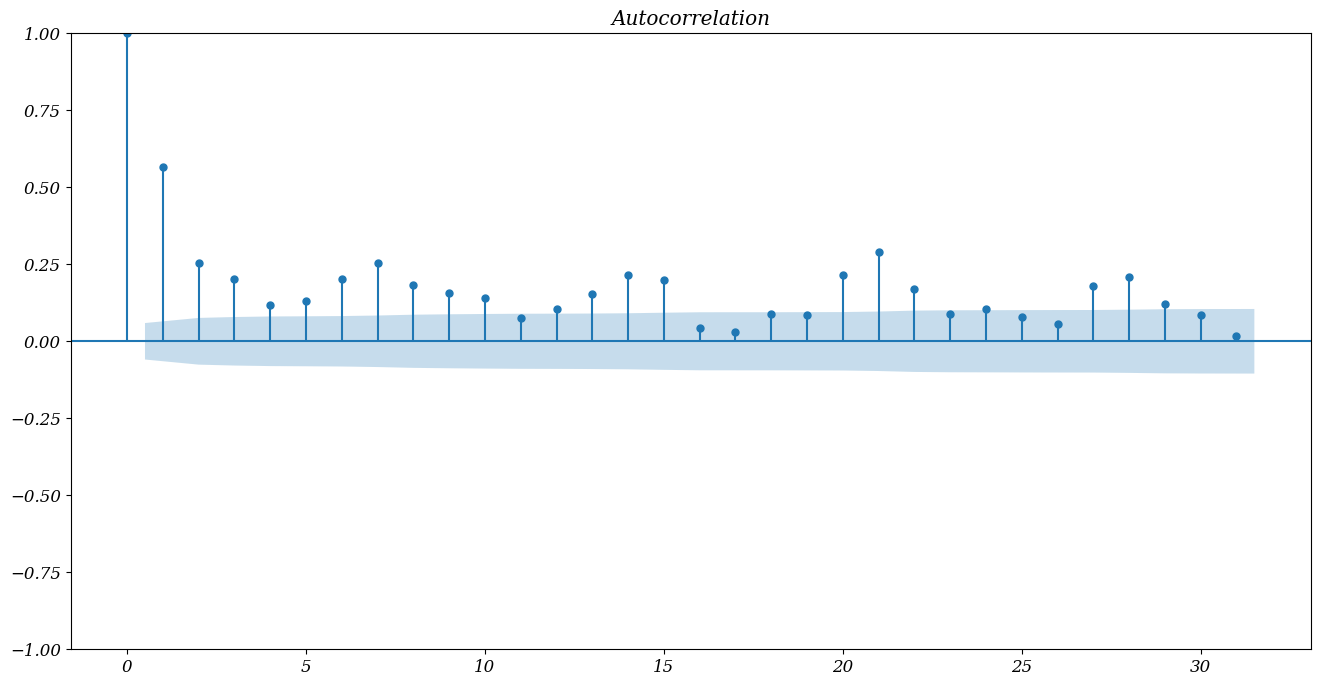
\includegraphics[width=0.5\linewidth]{Resultados/Figuras/acf} \qquad
	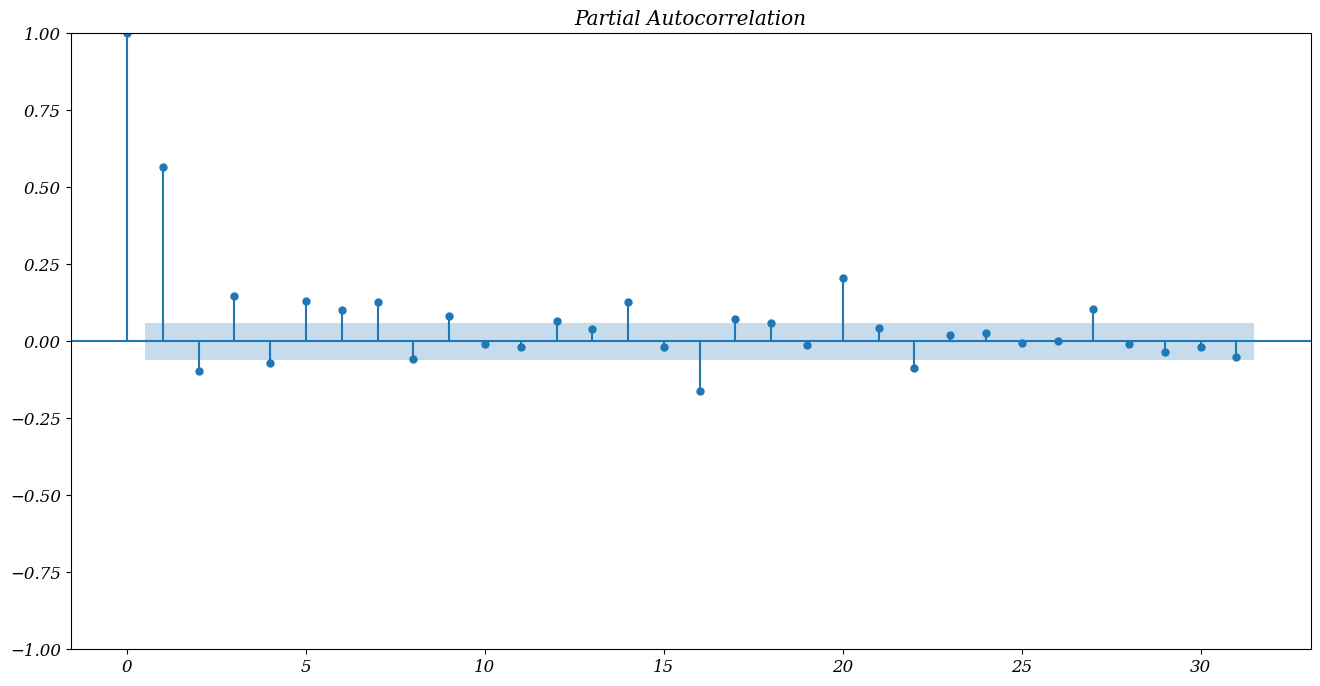
\includegraphics[width=0.5\linewidth]{Resultados/Figuras/pacf}
\end{minipage}
	Fonte: Elaboração própria a partir de dados da SANEPAR (2018 a 2020)
\end{figure}

Na Figura \ref{fig:acf} tem a diferença entre a autocorrelação e a autocorrelação parcial (PACF) é quase um detalhe em uma ACF temos a correlação direta e indireta e em uma PACF apenas a correlação direta. 

O intervalo de confiança por padrão é 95\%, mostrado como essa marca azul. Observações que estão para fora da marca são consideradas estatisticamente correlacionadas.

As correlação da Figura \ref{fig:acf} é a explicação do teste de DF, entendo isso pode ser visto o próximo passo que é  a análise do ruído branco em meados a gráfico, Uma série ruído branco é uma série na qual a média 0, a variância é constante ao longo da série toda e não há correlação entre os períodos de tempo. O valores de uma série ruídos brancos são totalmente aleatórios, ou seja, essa é um tipo de série que não é previsível.

\begin{figure}[H]
	\centering
	\caption{Ruído branco}
	\label{fig:ruido-branco}
	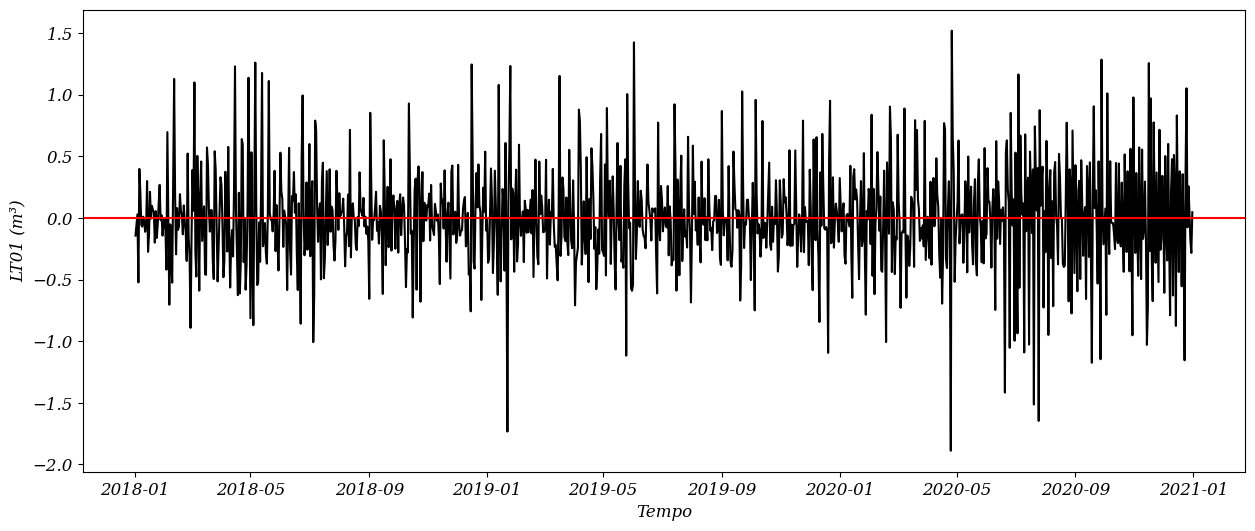
\includegraphics[width=1\linewidth]{Resultados/Figuras/ruido-branco}
	
	Fonte: Elaboração própria a partir de dados da SANEPAR (2018 a 2020)
\end{figure}

Da Figura \ref{fig:ruido-branco} uma série temporal pode ser ruído branco.
Uma série temporal é ruído branco se as variáveis são independentes e distribuídas de forma idêntica com uma média de zero.
Isso significa que todas as variáveis têm a mesma variância ($\sigma^2$) e cada valor tem uma correlação zero com todos os outros valores da série.
Mais para frente vamos mostrar o comprimento de zeros na variável prevista. Com isso encerra a \ref{etp:3}.

\subsubsection{Separação dos Dados}

Na \ref{etp:4} tem um esquema de como foi dividido os dados em treino, teste e validação, essa pratica é comum para os profissionais de aprendizado de máquina, pois assim como não é passível processar os dados todos de uma vez, se você manosear dados em uma escala menor até pode ser realizado, mas tudo depende da máquina que esta sendo realizado o processamento dos dados, cada modelo em particular utiliza um certo acervo do seu computador para processar, se por exemplo você tiver trabalhando com um modelo de aprendizado profundo que é mais comum em processamento de imagem, a Nvidia tem sempre inovado com as suas GPUs e trazendo mais poder para processamento, com o recente lançamento da placa de vídeo $3090$ um sonho de consumo para games e os profissionais de aprendizado de maquina e profundo.

Em fim se o computador que foi realizado os processamento fosse um computador não tão bom, ainda poderia está sendo pensando que estaria em processamento, sem as inovação que foi estabelecida aos anos, o computador que foi realizado os cálculos dos modelos foi em partes um computador de processador $i5-3300$ e um notebook com $i7-5500$ ambos com 4 threads e o notebook com apenas 2 núcleos o $i5$ contem 4 núcleos. Cada um tem suas especificações de ser o melhor em algum certo ponto, mas sabendo que não é preciso de um de ultima geração para fazer tais processamento. E sim força de vontade para entende e aplicar em cada um.

A divisão mais básica que tem na literatura foi realizada aqui na separação dos dados, $70\%$ para treino e os $30\%$ restante para teste, dos $70\%$ tem mais uma divisão pegando $80\%$ dos $70\%$ para treino novamente e os $20\%$ para validação dos dados, tendo essa fórmula aplica na linguagem de programação para que não precisa ser contado todas as vezes que for mudado o modelo.

\subsubsection{Estrategia de Previsão}\label{subsubsec:est}

Na \ref{etp:5} é abordado a forma que foi previsto os dados, em uma janela de horizonte de previsão bem maior do que o normal na literatura da estrategia de recursiva, sendo 1, 10, 30 e 60 dias previsto, essa estrategia para comparação dos modelos regressivo e modelos ARIMA, é bem vantajoso, pois cada modelo tem suas especificidade para prever em momentos com janela de tempo menor e com uma janela de muitos dias. Assim como explicado na seção \ref{subsubsec:modelos} se for previsão curta, alguns vai se sobre por em meio à outros modelos que foi feito aqui.

\subsubsection{Horizonte}

Na \ref{etp:6} é feito o horizonte de previsão, como dito na seção \ref{subsubsec:est} esse horizonte foi customizado baseado do método recursivo de prever as series temporais e a previsão do nível do tanque LT01. Os passos para prever a frente foi de 1, 10, 30 e 60 dias, já foi realizado uma estrategia com uma janela menor, mas para comparação dos modelos essa janela foi mais adequada.

\subsubsection{Modelos de previsão e métricas de desempenho}\label{subsubsec:modelos}

Da \ref{etp:7} as métricas utilizada aqui foi vista na seção \ref{subsec:metrica} foi utilizado aqui três das métricas mais usada na literaturar para previsão de tempo e comparação de modelos ARIMA e os modelos regressores.

    Em comparação com os modelos feito, pode ser visto que o modelo LR em um passo a frente tem tanto na modelagem de 24 horas quanto no pico de horas entre as 18 e 21 horas, foi o modelo que mais se saiu bem na previsão, logo em sequência os modelos MA, AR, SARIMA, ARIMA, SARIMAX, ARIMAX, ARX, LGBMRegressor, XGBRegressor e Random Forest Regressor, para curto prazo esses modelos estão em ordem de melhor para pior.
    
    Já em grande espaço de tempo como foi feito de 60 dias os modelos ARMA, AR, MA, ARIMA, ARIMAX, ARX, SARIMAX, SARIMA, XGBRegressor, Random Forest Regressor, LGBMRregressor e LR, seguindo a mesma lógica do melhor para o pior. Mas se olhar graficamente nos modelos que foi feito, os modelos com variáveis exógenas aparenta prever melhor do que os outros modelos, só analisando os dados nos apêndice tanto quando as Figuras de \ref{fig:1-AR-ARX-MA} a \ref{fig:60-LR-XGB-LGBM-RF24} quanto as Tabalas \ref{tb:1-24trn} a \ref{tb:60-18cm}   
    
    \subsubsection{Teste de Significância}
    
    Na \ref{etp:9} os teste escolhido foi de \textit{Friedman e Nemenjy} no teste de Nemenyi, precisamos obter a diferença entre os rankings médios (linha média da tabela de classificação) entre todos os classificadores (comparando pares de classificadores). Se essa diferença for maior ou igual a um CD (distância crítica), podemos dizer que esses dois classificadores são significativamente diferentes um do outro. O CD é calculado como:
    
    \begin{eqnarray}
    	C D&=&q_\alpha \sqrt{\frac{k(k+1)}{6 N}}\label{eq:neme}
    \end{eqnarray}

De \eqref{eq:neme} o termo $q_\alpha$ é obtido de ($\alpha=0,05$):

\begin{table}[H]
	\centering
	\caption{Teste Nemenyi}
	\begin{tabular}{@{}clllllllll@{}}
		\toprule
		\multicolumn{1}{l}{\textbf{Nemenyi}} & \multicolumn{1}{c}{\textbf{0}} & \multicolumn{1}{c}{\textbf{1}} & \multicolumn{1}{c}{\textbf{2}} & \multicolumn{1}{c}{\textbf{3}} & \multicolumn{1}{c}{\textbf{4}} & \multicolumn{1}{c}{\textbf{5}} & \multicolumn{1}{c}{\textbf{6}} & \multicolumn{1}{c}{\textbf{7}} & \multicolumn{1}{c}{\textbf{8}} \\ \midrule
		\textbf{0}                           & 1,000                          & 0,001                          & 0,001                          & 0,001                          & 0,001                          & 0,001                          & 0,001                          & 0,001                          & 0,001                          \\
		\textbf{1}                           & 0,001                          & 1,000                          & 0,001                          & 0,001                          & 0,001                          & 0,001                          & 0,001                          & 0,001                          & 0,157                          \\
		\textbf{2}                           & 0,001                          & 0,001                          & 1,000                          & 0,847                          & 0,001                          & 0,001                          & 0,001                          & 0,001                          & 0,001                          \\
		\textbf{3}                           & 0,001                          & 0,001                          & 0,847                          & 1,000                          & 0,001                          & 0,001                          & 0,001                          & 0,001                          & 0,001                          \\
		\textbf{4}                           & 0,001                          & 0,001                          & 0,001                          & 0,001                          & 1,000                          & 0,001                          & 0,001                          & 0,001                          & 0,001                          \\
		\textbf{5}                           & 0,001                          & 0,001                          & 0,001                          & 0,001                          & 0,001                          & 1,000                          & 0,001                          & 0,001                          & 0,001                          \\
		\textbf{6}                           & 0,001                          & 0,001                          & 0,001                          & 0,001                          & 0,001                          & 0,001                          & 1,000                          & 0,001                          & 0,001                          \\
		\textbf{7}                           & 0,001                          & 0,001                          & 0,001                          & 0,001                          & 0,001                          & 0,001                          & 0,001                          & 1,000                          & 0,001                          \\
		\textbf{8}                           & 0,001                          & 0,157                          & 0,001                          & 0,001                          & 0,001                          & 0,001                          & 0,001                          & 0,001                          & 1,000                          \\ \bottomrule
	\end{tabular}

Fonte: Elaboração própria a partir de dados da SANEPAR (2018 a 2020)
\end{table}

O teste de Nemenyi (Nemenyi, 1963) é um teste \textit{post-hoc}, ou seja, é um teste de comparação múltipla que é usado após a aplicação de teste não paramétricos com três ou mais fatores.
    
Para calcular a estatística de teste $F_r$ de Friedman cria-se inicialmente uma tabela com os dados, colocando-se em cada linha uma amostra e cada coluna correspondendo a uma condição de teste. A seguir, as amostras ao longo das condições são ordenadas, da melhor situação para a pior. Se não houver empates, usa-se a equação \eqref{eq:fr} para determinar a estatística de teste $F_r$:

\begin{eqnarray}
	F_r&=&\left[\frac{12}{n k(k+1)} \sum_{i=1}^k R_i{ }^2\right]-3 n(k+1)\label{eq:fr}
\end{eqnarray}
  
  Na equação \eqref{eq:fr} $n$ é o número de linhas (ou amostras), $k$ é o número de colunas (ou condições) e $R_i$ é a soma dos postos da coluna (ou condição) $i$.   
 Seguindo a equação \eqref{eq:fr} têm o seguinte resultado nos dados da pesquisa.
 
 $statistic=8015.611,\ \ pvalue=0.0$ com o números de 26306 linhas x 9 colunas.
    

    
